\documentclass[10pt]{article}
\usepackage[margin=0.75in]{geometry}
\usepackage{amsmath,amssymb,booktabs,longtable,graphicx,xcolor}
\usepackage[hidelinks]{hyperref}
\graphicspath{{figures/}}
\setlength{\parindent}{0pt}
\setlength{\parskip}{0.45em}
\title{BC1 Equal-Temperature Known-Answer Diagnostic\\Projection-Free Controlled Integrator}
\author{Numerical audit report}
\date{9 September 2026}
\begin{document}
\maketitle

\section{Question and frozen decision rule}
For the canonical BC1 bath at $T_1=T_n=6$, the stationary Gibbs density is
invariant under phase reversal, while every $\sin\theta_j$ is odd. Therefore
$\langle\sin\theta_j\rangle=0$ exactly. The inherited SIMD calculation failed
this control with maximum $|z|=8.678$ at $n=25$ and $12.929$ at $n=100$.
The diagnostic repeats only BC1 with the controlled Cartesian implementation:
double precision, fixed $dt=5\times10^{-4}$, standard trigonometry, no
adaptive stepping, and no positive-action projection or floor.

The gate was frozen before production. The port is accepted only if the
spatial mean action is within 5\% of the SIMD reference and its relative
spatial range is no larger than the SIMD range. The sine control is assessed
both pointwise at $|z|>1.95996$ and simultaneously with a two-sided
Bonferroni threshold.

\section{Protocol and integrity}
For $n=25$, burn-in and measurement times were 2000 and 2000. For $n=100$,
they were 32000 and 2000. The sample interval was 0.01, producing 200001
profile samples per trajectory. Two base seeds and 256 trajectories per base
seed gave 512 independent trajectories at each chain length.

\begin{center}
\begin{tabular}{rrrrr}
\toprule
$n$ & base seeds & trajectories & samples/trajectory & integrity errors\\
\midrule
25 & 2026090825, 2026090826 & 512 & 200001 & 0\\
100 & 2026090900, 2026090901 & 512 & 200001 & 0\\
\bottomrule
\end{tabular}
\end{center}

All 426 frozen output hashes verified, and a fresh independent invocation of
the frozen analysis reproduced the saved JSON byte-for-byte.

\section{Primary result}
\begin{center}
\begin{tabular}{rrrrrr}
\toprule
$n$ & controlled max $|z|$ & SIMD max $|z|$ & pointwise failures & Bonf. critical & simultaneous test\\
\midrule
25 & 1.875 & 8.678 & 0/24 & 3.078 & PASS\\
100 & 2.984 & 12.929 & 5/99 & 3.478 & PASS\\
\bottomrule
\end{tabular}
\end{center}

At $n=25$, no bond fails even the uncorrected pointwise test. At $n=100$,
5 of 99 bonds exceed 1.95996, approximately the number expected by chance
under 99 pointwise 5\% tests, while the maximum $|z|=2.984$ remains below the
predeclared simultaneous threshold 3.478. Thus the exact zero-sine control
passes at both lengths under the controlled integrator.

\begin{figure}[ht]
\centering
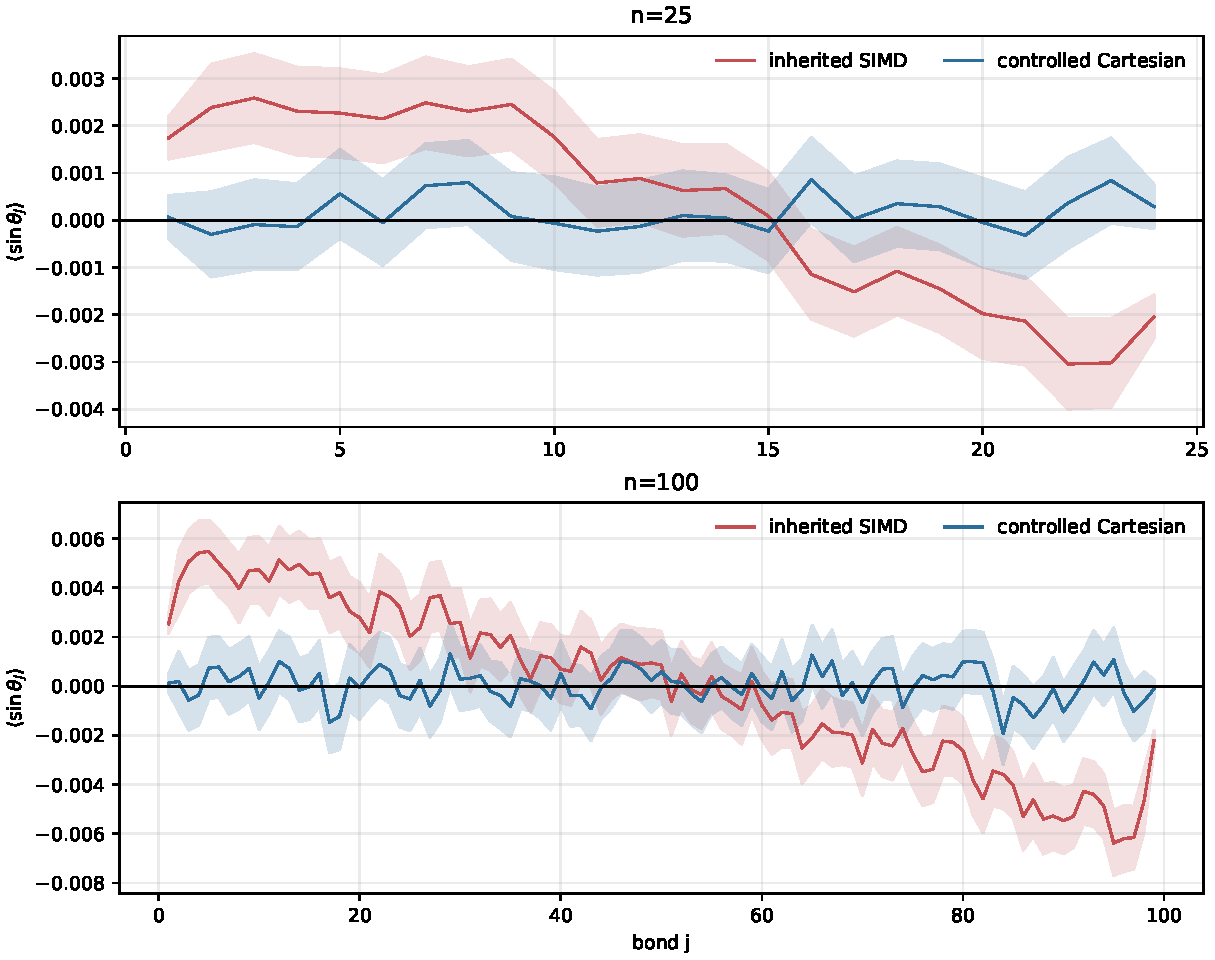
\includegraphics[width=0.94\textwidth]{bond_sine_profiles.pdf}
\caption{Bond-sine profiles and 95\% pointwise bands. The inherited SIMD
profile shows coherent nonzero structure; the controlled profile fluctuates
around zero.}
\end{figure}

\begin{figure}[ht]
\centering
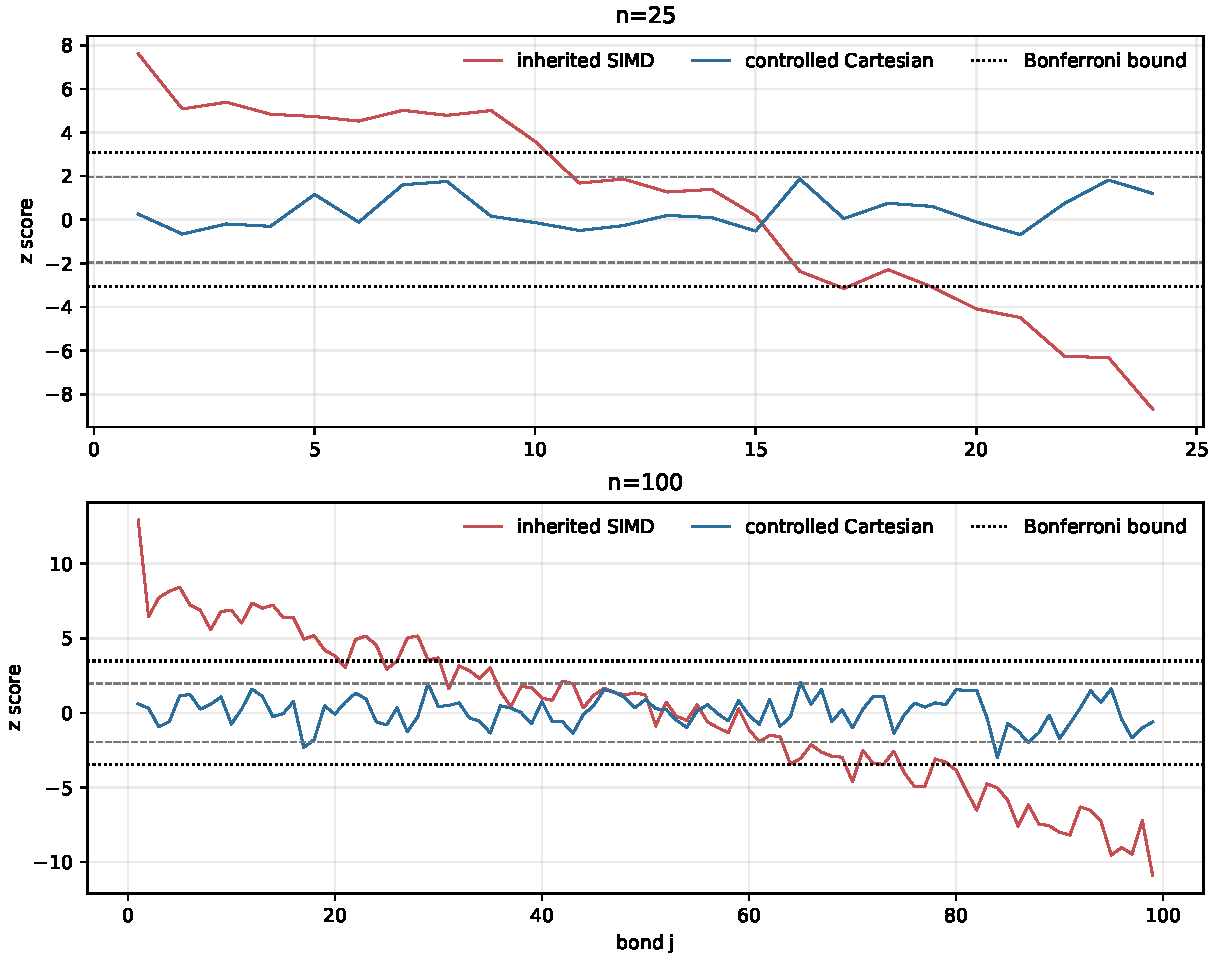
\includegraphics[width=0.94\textwidth]{bond_sine_z_scores.pdf}
\caption{Per-bond $z$ scores. Dotted lines are the frozen Bonferroni bounds;
dashed lines mark the uncorrected pointwise 95\% bounds.}
\end{figure}

\section{Like-for-like precision}
The mean controlled-to-SIMD SE ratios are comparable or smaller:
the median ratio is 0.979
at $n=25$ and 0.931 at
$n=100$. Mean controlled SEs are
0.000450711 and
0.000638362, compared with SIMD means
0.000459151 and
0.000687433. The disappearance of the coherent
signal is therefore not caused by reduced precision.

\section{Porting gate: action profile}
\begin{center}
\begin{tabular}{rrrrrr}
\toprule
$n$ & controlled mean & SIMD mean & relative difference & controlled range & SIMD range\\
\midrule
25 & 0.496684 & 0.494670 & 0.407\% & 0.706\% & 0.894\%\\
100 & 0.245984 & 0.249219 & 1.298\% & 1.725\% & 9.731\%\\
\bottomrule
\end{tabular}
\end{center}
Both predeclared porting gates pass. The spatial mean differs by only 0.407\%
at $n=25$ and 1.298\% at $n=100$, and the controlled profiles are flatter
than their SIMD references.

\begin{figure}[ht]
\centering
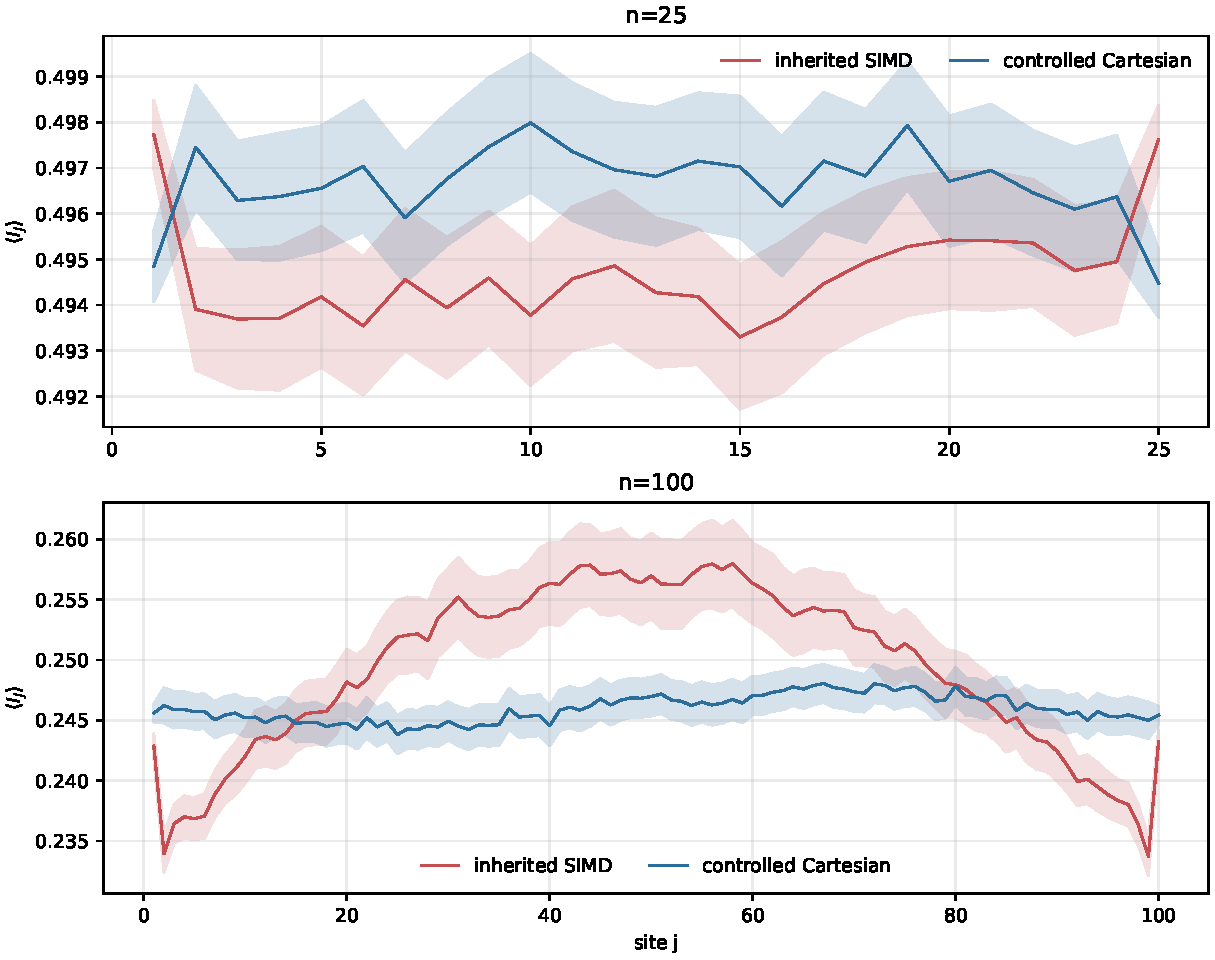
\includegraphics[width=0.94\textwidth]{action_profile_comparison.pdf}
\caption{Equal-temperature action profiles. The controlled port preserves
the action scale while eliminating the systematic bond-sine asymmetry.}
\end{figure}

\section{Numerical-event audit}
\begin{center}
\begin{tabular}{rrrrrr}
\toprule
$n$ & projections & floors & zero-radius & midpoint failures & min sampled action\\
\midrule
25 & 0 & 0 & 0 & 0 & 4.858175e-11\\
100 & 0 & 0 & 0 & 0 & 1.683034e-12\\
\bottomrule
\end{tabular}
\end{center}
Nonfinite batches were zero at both lengths. The near-zero-action region was
sampled down to $4.86\times10^{-11}$ and $1.68\times10^{-12}$ without
clipping.

\section{Verdict and claim boundary}
The controlled scheme passes the exact BC1 equal-temperature sine control at
both chain lengths, whereas the inherited SIMD scheme fails systematically at
comparable SE. Together with the passed action-profile porting gate, this
establishes that the old nonzero equal-temperature bond-sine profile is a
numerical artefact of the inherited SIMD numerical scheme, not a property of
the BC1 stationary dynamics. Because several numerical changes were made
together, this experiment does not identify projection alone as the unique
cause.

Consequently, driven $(10,2)$ bond-sine profiles obtained with the inherited
SIMD scheme should not be used quantitatively in the manuscript until they are
re-measured with the controlled integrator. Existing action-profile claims may
be retained subject to their separate validated gates.

\section{Provenance}
Launch commit: \nolinkurl{908a7c08faac7ea3b8eb06c0577fca7fb5e9ad5e}.\\
Remote frozen commit: \nolinkurl{35124a825a4119e9007c635e739ae71e3752d6b7}.\\
Source SHA-256: \nolinkurl{17d2b0e75c7838c7fc8710bae0f0381c7607c967d38e03b4db3bde34e8ec086b}.\\
Binary SHA-256: \nolinkurl{68c13863da721f655ecbd3d0913b80691c0a0a3a6c984877af8423c331c443db}.
The 64 unique completed production commands are preserved in the provenance
directory as \texttt{COMMANDS\_UNIQUE\_}\allowbreak\texttt{PRODUCTION.csv}.
The original \texttt{COMMANDS.csv} retains all 72 launch records, including eight
commands from the first detached attempt; that attempt produced no scientific
data and its empty logs are preserved under
\texttt{failed\_detached\_launch\_1}.

\clearpage
\appendix
\section{All bond-sine values}
\subsection{$n=25$}
\scriptsize
\begin{longtable}{rrrrrrr}
\toprule
$j$ & ctrl. mean & ctrl. SE & ctrl. $z$ & SIMD mean & SIMD SE & SIMD $z$\\
\midrule\endhead
1 & 6.15916e-05 & 0.00023579 & 0.26121 & 0.00174083 & 0.000228514 & 7.6181 \\
2 & -0.000300712 & 0.000460072 & -0.65362 & 0.00238436 & 0.000469214 & 5.0816 \\
3 & -9.25944e-05 & 0.000484063 & -0.19129 & 0.00258475 & 0.00047951 & 5.3904 \\
4 & -0.000138459 & 0.000463517 & -0.29871 & 0.00230554 & 0.000476456 & 4.8389 \\
5 & 0.000557895 & 0.000479749 & 1.1629 & 0.00226579 & 0.000478774 & 4.7325 \\
6 & -4.94622e-05 & 0.00046166 & -0.10714 & 0.0021442 & 0.000473771 & 4.5258 \\
7 & 0.000728997 & 0.000454126 & 1.6053 & 0.00248401 & 0.00049485 & 5.0197 \\
8 & 0.000796414 & 0.000453367 & 1.7567 & 0.00230344 & 0.000481128 & 4.7876 \\
9 & 7.73374e-05 & 0.000473886 & 0.1632 & 0.0024502 & 0.000489438 & 5.0062 \\
10 & -6.38396e-05 & 0.000500351 & -0.12759 & 0.00176292 & 0.000491034 & 3.5902 \\
11 & -0.000232355 & 0.000474126 & -0.49007 & 0.000788587 & 0.000468305 & 1.6839 \\
12 & -0.000132196 & 0.000495086 & -0.26702 & 0.00088276 & 0.000472852 & 1.8669 \\
13 & 9.77672e-05 & 0.000482694 & 0.20254 & 0.000628334 & 0.000493684 & 1.2727 \\
14 & 4.6572e-05 & 0.00046582 & 0.099979 & 0.000667911 & 0.000478831 & 1.3949 \\
15 & -0.000231863 & 0.000449133 & -0.51625 & 8.83032e-05 & 0.000476094 & 0.18547 \\
16 & 0.000855828 & 0.000456366 & 1.8753 & -0.00114343 & 0.000483543 & -2.3647 \\
17 & 2.56119e-05 & 0.000463101 & 0.055305 & -0.00151341 & 0.000480448 & -3.15 \\
18 & 0.000349486 & 0.000461511 & 0.75727 & -0.00107992 & 0.000472016 & -2.2879 \\
19 & 0.000284919 & 0.000463956 & 0.61411 & -0.00145148 & 0.000471163 & -3.0806 \\
20 & -4.80647e-05 & 0.000479285 & -0.10028 & -0.00197725 & 0.000484072 & -4.0846 \\
21 & -0.000319543 & 0.00046875 & -0.68169 & -0.002136 & 0.000476465 & -4.483 \\
22 & 0.000368907 & 0.000491523 & 0.75054 & -0.00304327 & 0.00048648 & -6.2557 \\
23 & 0.000837944 & 0.00046049 & 1.8197 & -0.00301796 & 0.000477369 & -6.3221 \\
24 & 0.000288455 & 0.000238637 & 1.2088 & -0.00204457 & 0.0002356 & -8.6781 \\
\bottomrule
\end{longtable}

\subsection{$n=100$}
\begin{longtable}{rrrrrrr}
\toprule
$j$ & ctrl. mean & ctrl. SE & ctrl. $z$ & SIMD mean & SIMD SE & SIMD $z$\\
\midrule\endhead
1 & 0.000117568 & 0.000193383 & 0.60795 & 0.00252443 & 0.00019526 & 12.929 \\
2 & 0.000190557 & 0.000621741 & 0.30649 & 0.00423771 & 0.000655634 & 6.4635 \\
3 & -0.000579927 & 0.000618558 & -0.93755 & 0.00505453 & 0.000654098 & 7.7275 \\
4 & -0.000364176 & 0.000622344 & -0.58517 & 0.00541257 & 0.00066381 & 8.1538 \\
5 & 0.000728779 & 0.000643359 & 1.1328 & 0.00547403 & 0.000649299 & 8.4307 \\
6 & 0.000776379 & 0.000624498 & 1.2432 & 0.00499207 & 0.000689233 & 7.2429 \\
7 & 0.000172189 & 0.000672839 & 0.25591 & 0.00454461 & 0.000660658 & 6.8789 \\
8 & 0.000387887 & 0.000674818 & 0.5748 & 0.00396825 & 0.000711925 & 5.574 \\
9 & 0.000712575 & 0.000662449 & 1.0757 & 0.00469443 & 0.000690576 & 6.7978 \\
10 & -0.000489026 & 0.000651363 & -0.75077 & 0.00472698 & 0.000687037 & 6.8802 \\
11 & 0.000170656 & 0.000655408 & 0.26038 & 0.00426106 & 0.00070687 & 6.0281 \\
12 & 0.0010045 & 0.000630471 & 1.5933 & 0.00513069 & 0.00069719 & 7.3591 \\
13 & 0.000716707 & 0.000645378 & 1.1105 & 0.00472077 & 0.000672774 & 7.0169 \\
14 & -0.000165989 & 0.000659296 & -0.25177 & 0.00495506 & 0.000685596 & 7.2274 \\
15 & -3.80497e-05 & 0.000672127 & -0.056611 & 0.004537 & 0.000708173 & 6.4066 \\
16 & 0.000512246 & 0.000680137 & 0.75315 & 0.00458986 & 0.000718993 & 6.3837 \\
17 & -0.00147243 & 0.000634706 & -2.3199 & 0.0035845 & 0.000723534 & 4.9542 \\
18 & -0.00123338 & 0.000688561 & -1.7912 & 0.0037957 & 0.000732921 & 5.1789 \\
19 & 0.000327251 & 0.00069286 & 0.47232 & 0.0030392 & 0.000720766 & 4.2166 \\
20 & -5.31348e-05 & 0.000660133 & -0.080491 & 0.00277851 & 0.000725791 & 3.8282 \\
21 & 0.000482462 & 0.000672692 & 0.71721 & 0.00216696 & 0.000712798 & 3.0401 \\
22 & 0.000881731 & 0.000667885 & 1.3202 & 0.003832 & 0.000777342 & 4.9296 \\
23 & 0.000633444 & 0.000673031 & 0.94118 & 0.00362704 & 0.000704465 & 5.1486 \\
24 & -0.000389442 & 0.000651547 & -0.59772 & 0.00319663 & 0.000705255 & 4.5326 \\
25 & -0.000528584 & 0.000655713 & -0.80612 & 0.00202013 & 0.000688746 & 2.9331 \\
26 & 0.000227436 & 0.000671807 & 0.33854 & 0.00237325 & 0.000682061 & 3.4795 \\
27 & -0.000812819 & 0.000642493 & -1.2651 & 0.00359058 & 0.000714531 & 5.0251 \\
28 & -0.000172894 & 0.000661013 & -0.26156 & 0.0036809 & 0.000713195 & 5.1611 \\
29 & 0.00130636 & 0.000665555 & 1.9628 & 0.00253569 & 0.000714524 & 3.5488 \\
30 & 0.000276185 & 0.000651829 & 0.42371 & 0.00259444 & 0.000702842 & 3.6913 \\
31 & 0.000322316 & 0.00064058 & 0.50316 & 0.00113833 & 0.000704793 & 1.6151 \\
32 & 0.000425434 & 0.000635262 & 0.6697 & 0.00215534 & 0.0006841 & 3.1506 \\
33 & -0.000212748 & 0.00062014 & -0.34306 & 0.00209149 & 0.000738228 & 2.8331 \\
34 & -0.00038509 & 0.000688476 & -0.55934 & 0.00157067 & 0.00068372 & 2.2972 \\
35 & -0.000841117 & 0.000625408 & -1.3449 & 0.00206326 & 0.000682449 & 3.0233 \\
36 & 0.000297027 & 0.000623805 & 0.47615 & 0.00105026 & 0.000735386 & 1.4282 \\
37 & 0.000197912 & 0.000615865 & 0.32136 & 0.000287079 & 0.00069118 & 0.41535 \\
38 & 1.21658e-05 & 0.000680466 & 0.017879 & 0.00122992 & 0.000689357 & 1.7842 \\
39 & -0.000483625 & 0.000666368 & -0.72576 & 0.0011479 & 0.000681918 & 1.6833 \\
40 & 0.000515675 & 0.000675597 & 0.76329 & 0.000683053 & 0.000696702 & 0.98041 \\
41 & -0.000380527 & 0.000643252 & -0.59157 & 0.000600037 & 0.000704547 & 0.85166 \\
42 & -0.000369708 & 0.000616754 & -0.59944 & 0.00158496 & 0.000743578 & 2.1315 \\
43 & -0.00092201 & 0.000667803 & -1.3807 & 0.00133733 & 0.00068344 & 1.9568 \\
44 & -6.86376e-05 & 0.000649934 & -0.10561 & 0.000242726 & 0.000713261 & 0.3403 \\
45 & 0.000301071 & 0.000617322 & 0.48771 & 0.000816815 & 0.000691317 & 1.1815 \\
46 & 0.00100712 & 0.000644246 & 1.5633 & 0.00115351 & 0.000695826 & 1.6578 \\
47 & 0.000937978 & 0.000673311 & 1.3931 & 0.000982132 & 0.000717265 & 1.3693 \\
48 & 0.000687269 & 0.000656111 & 1.0475 & 0.000884114 & 0.000732792 & 1.2065 \\
49 & 0.000230016 & 0.00066138 & 0.34778 & 0.00094038 & 0.000700969 & 1.3415 \\
50 & 0.000580777 & 0.000646192 & 0.89877 & 0.00085233 & 0.000702686 & 1.213 \\
51 & 0.000179482 & 0.000658228 & 0.27268 & -0.000617296 & 0.000703657 & -0.87727 \\
52 & 0.000150586 & 0.000671548 & 0.22424 & 0.000488491 & 0.000677706 & 0.7208 \\
53 & -0.000317661 & 0.000636594 & -0.499 & -0.000162594 & 0.000681147 & -0.23871 \\
54 & -0.000628833 & 0.000649377 & -0.96836 & -0.000342281 & 0.000699912 & -0.48903 \\
55 & 8.9059e-05 & 0.000622296 & 0.14311 & 0.000385899 & 0.000706267 & 0.54639 \\
56 & 0.000346581 & 0.000633688 & 0.54693 & -0.000414589 & 0.000679654 & -0.61 \\
57 & -3.48977e-05 & 0.000646388 & -0.053989 & -0.000668478 & 0.000675302 & -0.9899 \\
58 & -0.000344593 & 0.00063773 & -0.54034 & -0.000953963 & 0.000718607 & -1.3275 \\
59 & 0.000505914 & 0.000608927 & 0.83083 & 0.000191546 & 0.000703281 & 0.27236 \\
60 & -0.000114545 & 0.000679867 & -0.16848 & -0.000780364 & 0.000705091 & -1.1068 \\
61 & -0.000500066 & 0.00065297 & -0.76583 & -0.00138258 & 0.000709662 & -1.9482 \\
62 & 0.000591755 & 0.000661437 & 0.89465 & -0.00107066 & 0.00071652 & -1.4942 \\
63 & -0.000586066 & 0.000656244 & -0.89306 & -0.00111601 & 0.00070029 & -1.5936 \\
64 & -0.000167381 & 0.000638575 & -0.26212 & -0.00251716 & 0.000734295 & -3.428 \\
65 & 0.00125866 & 0.000617364 & 2.0388 & -0.00210191 & 0.000690059 & -3.046 \\
66 & 0.000378213 & 0.000655416 & 0.57706 & -0.00153359 & 0.000718302 & -2.135 \\
67 & 0.00101519 & 0.000646203 & 1.571 & -0.00186727 & 0.000711234 & -2.6254 \\
68 & -0.000378219 & 0.000654799 & -0.57761 & -0.00190585 & 0.000656278 & -2.904 \\
69 & 0.000137089 & 0.000646653 & 0.212 & -0.00198338 & 0.000667741 & -2.9703 \\
70 & -0.000683677 & 0.00067842 & -1.0077 & -0.00313011 & 0.000677459 & -4.6204 \\
71 & 0.000157577 & 0.000636902 & 0.24741 & -0.00175454 & 0.000694355 & -2.5269 \\
72 & 0.000686884 & 0.000633077 & 1.085 & -0.00232683 & 0.000685714 & -3.3933 \\
73 & 0.000727343 & 0.000654107 & 1.112 & -0.00243385 & 0.000706558 & -3.4446 \\
74 & -0.000861578 & 0.000626894 & -1.3744 & -0.00172796 & 0.000674 & -2.5637 \\
75 & -9.30401e-05 & 0.000663201 & -0.14029 & -0.0027519 & 0.000686047 & -4.0112 \\
76 & 0.000433919 & 0.000657679 & 0.65977 & -0.00348594 & 0.000704613 & -4.9473 \\
77 & 0.000252005 & 0.000648226 & 0.38876 & -0.00338458 & 0.000690821 & -4.8994 \\
78 & 0.000439137 & 0.000651315 & 0.67423 & -0.0022334 & 0.000723739 & -3.0859 \\
79 & 0.000371229 & 0.000670488 & 0.55367 & -0.00228106 & 0.000689895 & -3.3064 \\
80 & 0.000983498 & 0.000634222 & 1.5507 & -0.00261721 & 0.000681222 & -3.8419 \\
81 & 0.000985679 & 0.000650189 & 1.516 & -0.00381041 & 0.000729565 & -5.2229 \\
82 & 0.00094879 & 0.000631328 & 1.5028 & -0.00458439 & 0.000704097 & -6.511 \\
83 & -0.000224551 & 0.000661633 & -0.33939 & -0.00345404 & 0.000726089 & -4.7571 \\
84 & -0.00192651 & 0.000645606 & -2.984 & -0.00358658 & 0.000713924 & -5.0238 \\
85 & -0.000460093 & 0.000647649 & -0.7104 & -0.00402858 & 0.000688539 & -5.8509 \\
86 & -0.000762082 & 0.000619863 & -1.2294 & -0.00530198 & 0.000698177 & -7.594 \\
87 & -0.00128713 & 0.00064364 & -1.9998 & -0.0046297 & 0.000750655 & -6.1675 \\
88 & -0.000784828 & 0.000591597 & -1.3266 & -0.00540516 & 0.000726234 & -7.4427 \\
89 & -9.42562e-05 & 0.000642759 & -0.14664 & -0.00528334 & 0.000698217 & -7.5669 \\
90 & -0.00105221 & 0.000607964 & -1.7307 & -0.00547441 & 0.000684336 & -7.9996 \\
91 & -0.000460395 & 0.000640498 & -0.71881 & -0.00529657 & 0.000646573 & -8.1917 \\
92 & 0.000197691 & 0.000620125 & 0.31879 & -0.00427971 & 0.000678497 & -6.3076 \\
93 & 0.000973932 & 0.000655188 & 1.4865 & -0.00439924 & 0.000673234 & -6.5345 \\
94 & 0.000451858 & 0.000639976 & 0.70605 & -0.00486309 & 0.000668534 & -7.2743 \\
95 & 0.00106967 & 0.000659678 & 1.6215 & -0.00638756 & 0.000670078 & -9.5326 \\
96 & -0.000260969 & 0.000623204 & -0.41875 & -0.00619381 & 0.000686272 & -9.0253 \\
97 & -0.0010299 & 0.000613709 & -1.6782 & -0.00615973 & 0.000651003 & -9.4619 \\
98 & -0.000617765 & 0.000616082 & -1.0027 & -0.00469157 & 0.000649136 & -7.2274 \\
99 & -0.000116681 & 0.000192011 & -0.60768 & -0.00222266 & 0.000203852 & -10.903 \\
\bottomrule
\end{longtable}

\clearpage
\section{Full action profiles}
\subsection{$n=25$}
\begin{longtable}{rrrrrr}
\toprule
$j$ & ctrl. mean & ctrl. SE & SIMD mean & SIMD SE & difference\\
\midrule\endhead
1 & 0.494851 & 0.00039856 & 0.497723 & 0.000385703 & -0.00287251 \\
2 & 0.497451 & 0.000688705 & 0.493908 & 0.000676646 & 0.00354322 \\
3 & 0.496289 & 0.000662098 & 0.493696 & 0.000771049 & 0.00259274 \\
4 & 0.496372 & 0.000708227 & 0.49371 & 0.00080127 & 0.00266255 \\
5 & 0.496555 & 0.000694966 & 0.494181 & 0.000784706 & 0.00237355 \\
6 & 0.497034 & 0.000734785 & 0.493545 & 0.00076985 & 0.0034886 \\
7 & 0.49591 & 0.000723452 & 0.494559 & 0.000791412 & 0.00135146 \\
8 & 0.496757 & 0.000739303 & 0.49394 & 0.000786145 & 0.00281646 \\
9 & 0.497461 & 0.000771285 & 0.494593 & 0.000745615 & 0.00286732 \\
10 & 0.497986 & 0.000772239 & 0.493775 & 0.000779022 & 0.00421113 \\
11 & 0.497356 & 0.000767663 & 0.494574 & 0.000803053 & 0.00278162 \\
12 & 0.49696 & 0.000751841 & 0.494858 & 0.000842878 & 0.00210182 \\
13 & 0.496815 & 0.000769919 & 0.494271 & 0.000833112 & 0.00254406 \\
14 & 0.49715 & 0.000762312 & 0.494186 & 0.000758871 & 0.00296353 \\
15 & 0.497024 & 0.000788579 & 0.493303 & 0.000804662 & 0.00372096 \\
16 & 0.496164 & 0.000778576 & 0.493735 & 0.000843669 & 0.002429 \\
17 & 0.49715 & 0.000768223 & 0.494467 & 0.000794466 & 0.00268287 \\
18 & 0.496824 & 0.000741647 & 0.494941 & 0.000789197 & 0.00188295 \\
19 & 0.497927 & 0.000713704 & 0.495279 & 0.000769403 & 0.00264835 \\
20 & 0.496708 & 0.000727566 & 0.495421 & 0.000765069 & 0.00128641 \\
21 & 0.496948 & 0.000738684 & 0.495408 & 0.000777104 & 0.0015407 \\
22 & 0.496456 & 0.000696039 & 0.495359 & 0.00070798 & 0.00109697 \\
23 & 0.496099 & 0.000690713 & 0.494756 & 0.000723627 & 0.00134282 \\
24 & 0.49637 & 0.000685763 & 0.494949 & 0.000683413 & 0.00142065 \\
25 & 0.494477 & 0.000377816 & 0.497615 & 0.000383806 & -0.00313807 \\
\bottomrule
\end{longtable}

\subsection{$n=100$}
\begin{longtable}{rrrrrr}
\toprule
$j$ & ctrl. mean & ctrl. SE & SIMD mean & SIMD SE & difference\\
\midrule\endhead
1 & 0.245591 & 0.000384898 & 0.242864 & 0.00051366 & 0.00272724 \\
2 & 0.246234 & 0.000743112 & 0.233955 & 0.000793743 & 0.012279 \\
3 & 0.245871 & 0.000768108 & 0.236451 & 0.00081271 & 0.00942019 \\
4 & 0.245893 & 0.000747673 & 0.237009 & 0.000885779 & 0.00888423 \\
5 & 0.245714 & 0.000739662 & 0.236853 & 0.000885459 & 0.00886044 \\
6 & 0.245741 & 0.000735928 & 0.237079 & 0.000941077 & 0.00866176 \\
7 & 0.245043 & 0.000764052 & 0.238866 & 0.000983273 & 0.0061765 \\
8 & 0.245433 & 0.000778844 & 0.240107 & 0.00101802 & 0.0053259 \\
9 & 0.245602 & 0.00077765 & 0.24094 & 0.00109773 & 0.00466192 \\
10 & 0.245205 & 0.000797061 & 0.242026 & 0.00114398 & 0.00317876 \\
11 & 0.245266 & 0.000799172 & 0.243421 & 0.00122329 & 0.00184472 \\
12 & 0.244792 & 0.000817969 & 0.243661 & 0.00125013 & 0.00113173 \\
13 & 0.245222 & 0.000820276 & 0.243382 & 0.00120569 & 0.00183973 \\
14 & 0.245346 & 0.000802805 & 0.243907 & 0.00125345 & 0.00143902 \\
15 & 0.244739 & 0.000783658 & 0.244997 & 0.00129757 & -0.000257423 \\
16 & 0.244841 & 0.000791479 & 0.245561 & 0.00135769 & -0.00072039 \\
17 & 0.244842 & 0.000835804 & 0.245662 & 0.00136355 & -0.000820182 \\
18 & 0.244475 & 0.000829075 & 0.245726 & 0.00137333 & -0.00125176 \\
19 & 0.244667 & 0.00082716 & 0.246744 & 0.00143368 & -0.00207663 \\
20 & 0.244765 & 0.000835011 & 0.248172 & 0.00137957 & -0.00340751 \\
21 & 0.244244 & 0.000829844 & 0.247702 & 0.00138695 & -0.00345847 \\
22 & 0.245214 & 0.000857684 & 0.248387 & 0.00138951 & -0.00317378 \\
23 & 0.244452 & 0.000812871 & 0.249859 & 0.00145652 & -0.0054078 \\
24 & 0.244879 & 0.000797714 & 0.251052 & 0.00150613 & -0.00617363 \\
25 & 0.243806 & 0.000814215 & 0.251893 & 0.00155246 & -0.00808693 \\
26 & 0.2443 & 0.00080605 & 0.252053 & 0.00161005 & -0.00775311 \\
27 & 0.244224 & 0.000819625 & 0.252154 & 0.0015493 & -0.00792919 \\
28 & 0.244554 & 0.000830094 & 0.251602 & 0.00160974 & -0.00704782 \\
29 & 0.244443 & 0.000827385 & 0.253476 & 0.00162879 & -0.00903287 \\
30 & 0.244936 & 0.000810498 & 0.25432 & 0.00165933 & -0.00938373 \\
31 & 0.244515 & 0.000821231 & 0.255206 & 0.00168757 & -0.010691 \\
32 & 0.244235 & 0.000852017 & 0.254279 & 0.00167128 & -0.0100441 \\
33 & 0.244613 & 0.00084461 & 0.253626 & 0.00166095 & -0.0090134 \\
34 & 0.244591 & 0.000884093 & 0.253518 & 0.00168594 & -0.00892668 \\
35 & 0.244628 & 0.000865443 & 0.25364 & 0.00169136 & -0.00901202 \\
36 & 0.245962 & 0.000855924 & 0.254159 & 0.00163474 & -0.00819623 \\
37 & 0.245265 & 0.000867089 & 0.25427 & 0.0015816 & -0.0090043 \\
38 & 0.245344 & 0.000860437 & 0.255002 & 0.00161408 & -0.00965865 \\
39 & 0.24542 & 0.000867503 & 0.255991 & 0.00165187 & -0.0105709 \\
40 & 0.244542 & 0.000843892 & 0.256344 & 0.00172423 & -0.0118022 \\
41 & 0.24584 & 0.000859357 & 0.256258 & 0.00174581 & -0.0104174 \\
42 & 0.246086 & 0.000866315 & 0.257107 & 0.00176384 & -0.0110218 \\
43 & 0.245842 & 0.000879005 & 0.257808 & 0.00176468 & -0.0119658 \\
44 & 0.246186 & 0.000857395 & 0.257852 & 0.00169924 & -0.0116656 \\
45 & 0.246775 & 0.000850343 & 0.257112 & 0.00169358 & -0.0103372 \\
46 & 0.246271 & 0.000850042 & 0.25714 & 0.00176151 & -0.0108691 \\
47 & 0.246664 & 0.000837398 & 0.257372 & 0.00177978 & -0.0107077 \\
48 & 0.246856 & 0.000821391 & 0.256671 & 0.00173245 & -0.00981456 \\
49 & 0.246831 & 0.000804652 & 0.256383 & 0.00177066 & -0.0095518 \\
50 & 0.246962 & 0.000816301 & 0.256962 & 0.00181343 & -0.010001 \\
51 & 0.247171 & 0.000818389 & 0.256287 & 0.0018637 & -0.00911631 \\
52 & 0.246684 & 0.000813361 & 0.256265 & 0.00187104 & -0.00958139 \\
53 & 0.246571 & 0.000828858 & 0.256238 & 0.00185207 & -0.00966723 \\
54 & 0.246223 & 0.000838815 & 0.257083 & 0.00180099 & -0.0108596 \\
55 & 0.246509 & 0.000852541 & 0.257727 & 0.00180411 & -0.0112185 \\
56 & 0.246271 & 0.000852303 & 0.25794 & 0.00185795 & -0.0116689 \\
57 & 0.246412 & 0.000845726 & 0.257492 & 0.0017903 & -0.0110793 \\
58 & 0.24672 & 0.000847968 & 0.257978 & 0.00181781 & -0.0112583 \\
59 & 0.246434 & 0.000840399 & 0.257168 & 0.00179479 & -0.0107341 \\
60 & 0.247059 & 0.000812533 & 0.256351 & 0.00170143 & -0.00929281 \\
61 & 0.247076 & 0.000812529 & 0.255882 & 0.00170103 & -0.00880573 \\
62 & 0.247325 & 0.000803456 & 0.255303 & 0.0017453 & -0.00797854 \\
63 & 0.247458 & 0.000809496 & 0.254347 & 0.0016827 & -0.00688916 \\
64 & 0.247778 & 0.000791127 & 0.253665 & 0.00168362 & -0.00588719 \\
65 & 0.247582 & 0.000818681 & 0.254019 & 0.00174169 & -0.0064367 \\
66 & 0.247879 & 0.000814823 & 0.25434 & 0.00166599 & -0.00646066 \\
67 & 0.248051 & 0.000804635 & 0.254049 & 0.00161504 & -0.00599787 \\
68 & 0.247713 & 0.000846496 & 0.254117 & 0.00157771 & -0.00640385 \\
69 & 0.247591 & 0.000818257 & 0.254005 & 0.00156399 & -0.00641415 \\
70 & 0.247362 & 0.000831575 & 0.252677 & 0.00157658 & -0.00531534 \\
71 & 0.247244 & 0.000793397 & 0.252446 & 0.00150027 & -0.00520186 \\
72 & 0.248029 & 0.000804977 & 0.252315 & 0.00148956 & -0.00428674 \\
73 & 0.24789 & 0.000764393 & 0.251145 & 0.00146835 & -0.00325507 \\
74 & 0.247451 & 0.000780318 & 0.250766 & 0.00146245 & -0.00331539 \\
75 & 0.247706 & 0.000792669 & 0.251344 & 0.00145329 & -0.00363822 \\
76 & 0.247799 & 0.000809247 & 0.250743 & 0.00143293 & -0.00294437 \\
77 & 0.247326 & 0.000775163 & 0.249665 & 0.00141873 & -0.00233987 \\
78 & 0.246579 & 0.000770876 & 0.248847 & 0.00141902 & -0.00226796 \\
79 & 0.246691 & 0.000775043 & 0.248058 & 0.00143229 & -0.00136677 \\
80 & 0.24784 & 0.000781466 & 0.247958 & 0.00140661 & -0.000117306 \\
81 & 0.246961 & 0.00078699 & 0.247562 & 0.00144617 & -0.00060143 \\
82 & 0.246912 & 0.000798401 & 0.246889 & 0.00139643 & 2.33183e-05 \\
83 & 0.246609 & 0.000764735 & 0.246511 & 0.00128781 & 9.79083e-05 \\
84 & 0.247081 & 0.000768839 & 0.245741 & 0.00125995 & 0.00134057 \\
85 & 0.247014 & 0.000785425 & 0.244838 & 0.00126343 & 0.00217653 \\
86 & 0.245811 & 0.00077731 & 0.245223 & 0.00125223 & 0.000587729 \\
87 & 0.246389 & 0.00078037 & 0.244027 & 0.0012621 & 0.00236213 \\
88 & 0.246 & 0.000764941 & 0.243381 & 0.00124857 & 0.00261963 \\
89 & 0.245914 & 0.000786432 & 0.243193 & 0.00124649 & 0.00272094 \\
90 & 0.245925 & 0.00079273 & 0.242444 & 0.00124597 & 0.00348005 \\
91 & 0.245486 & 0.000784579 & 0.241279 & 0.00113532 & 0.00420712 \\
92 & 0.245682 & 0.000779679 & 0.239937 & 0.00101715 & 0.00574439 \\
93 & 0.245001 & 0.000777971 & 0.240117 & 0.00102936 & 0.00488387 \\
94 & 0.245743 & 0.00075825 & 0.239495 & 0.0010183 & 0.00624805 \\
95 & 0.245352 & 0.000776831 & 0.238852 & 0.000947308 & 0.00649981 \\
96 & 0.245272 & 0.000745491 & 0.238357 & 0.000894351 & 0.00691497 \\
97 & 0.245447 & 0.00076356 & 0.238032 & 0.000901977 & 0.00741563 \\
98 & 0.245233 & 0.000767487 & 0.236343 & 0.000856787 & 0.00889003 \\
99 & 0.244999 & 0.000770357 & 0.233726 & 0.000806154 & 0.0112737 \\
100 & 0.245406 & 0.000385367 & 0.243197 & 0.000510941 & 0.00220913 \\
\bottomrule
\end{longtable}
\end{document}
